\section{Certifying an improvement over a feasible schedule}
\label{sec:baselineexecution}

A bound on distance from an unknown optimum need not answer the immediate
execution question: should a proposed schedule replace the schedule already
in use? This section compares both schedules under the \emph{same} uncertain
cost law. Common uncertainty then cancels where the schedules agree.
Baseline-relative robust improvement is an established control principle
\citep{GhavamzadehPetrikChow2016}; convex trading formulations with explicit
costs and constraints are developed by \citet{BoydEtAl2017}. The result below
is an execution specialization: a box of temporary-impact coefficients and
an ellipsoid of linear charges give an exact, closed-form acceptance step
along a proposed, quantity-conserving schedule change.

\subsection{The mandate and the uncertainty set}

There are $n$ execution bins. Quantities have one common unit, and the buy
schedule belongs to
\[
 K=\{x\in\R^n: \mathbf1^\top x=Q,\ 0\le x_i\le u_i\},
 \qquad Q>0,\quad u_i\ge0,\quad \sum_i u_i\ge Q.
\]
The bounds are executable capacities in the declared model, not expected
passive fills. Let $b,x\in K$ be a baseline and a proposed schedule,
$d=x-b$, and $x(t)=b+td$, $0\le t\le1$. Every such schedule completes
the mandate and respects the same caps. Consider the family
\begin{equation}\label{eq:baselinefamily}
 C_{z,v}(y)=\tfrac12y^\top(H+\operatorname{diag}z)y
                  +(c+Bv)^\top y,
 \qquad |z_i|\le\epsilon_i,\quad \|v\|_2\le\rho.
\end{equation}
Here $H$ is symmetric, $H-\operatorname{diag}\epsilon\succeq0$,
and the box and ball form a Cartesian product. $H$ may contain a known
transient-impact or inventory-risk quadratic; only its diagonal correction
is uncertain. The linear charge can include fees or an adverse drift.
All costs are in the same units. The family is conditional on the information
available when this schedule comparison is made.

\begin{theorem}[Exact robust schedule step]\label{thm:baselinestep}
Define $\operatorname{sgn}(0)=0$ and
\begin{align}
 A_d&=d^\top(Hb+c)+\sum_i\epsilon_i b_i|d_i|
                        +\rho\|B^\top d\|_2,\label{eq:stepA}\\
 D_d&=d^\top H d+\sum_i\epsilon_i\operatorname{sgn}(d_i)d_i^2.
 \label{eq:stepD}
\end{align}
Then $D_d\ge0$ and, simultaneously for $0\le t\le1$,
\begin{equation}\label{eq:exactstep}
 \sup_{z,v}\{C_{z,v}(x(t))-C_{z,v}(b)\}
          = A_dt+\tfrac12D_dt^2=:\Psi_d(t).
\end{equation}
If $A_d\ge0$, $t_*=0$ minimizes this expression. If $A_d<0<D_d$,
its minimizer is $t_*=\min\{1,-A_d/D_d\}$; if $A_d<0=D_d$, it is
$t_*=1$. The accepted schedule satisfies, for every law in the family,
\[
 C_{z,v}(x(t_*))\le C_{z,v}(b)-G_d,\qquad
 G_d=-\Psi_d(t_*)\ge0.
\]
When $0<-A_d<D_d$, the guaranteed saving is $A_d^2/(2D_d)$.
\end{theorem}
\begin{proof}
Expand the cost difference in \eqref{eq:baselinefamily}. The uncertain
diagonal contribution is $\tfrac12\sum_i z_i((b_i+td_i)^2-b_i^2)$.
Because $b_i$ and $b_i+td_i$ are nonnegative, its coefficient has the sign
of $d_i$ for $t>0$ whenever it is nonzero. The maximizing corner is therefore
$z_i=\epsilon_i\operatorname{sgn}(d_i)$, independent of $t>0$.
Its contribution is
$t\sum_i\epsilon_i b_i|d_i|+\tfrac12t^2
\sum_i\epsilon_i\operatorname{sgn}(d_i)d_i^2$.
The support function of the ball gives
$\sup_{\|v\|\le\rho}tv^\top B^\top d=t\rho\|B^\top d\|$.
Independence of the uncertainty factors proves equality, including $t=0$.
The adverse diagonal matrix is positive semidefinite after addition to $H$,
so $D_d\ge0$. Minimizing this convex quadratic over $[0,1]$ proves the
remaining assertions. Convexity of $K$ proves feasibility.
\end{proof}

\begin{remark}[What is exact and what remains conditional]
The theorem optimizes the fraction of a supplied proposal; it does not solve
the globally optimal robust schedule problem. It is exact for the Cartesian
family in \eqref{eq:baselinefamily}; enlarging a correlated family to this
box and ellipsoid gives an upper bound, possibly conservative. Signed trades
can change the sign of the squared-quantity difference along the segment,
so the displayed single-quadratic formula cannot be used unchanged for
round trips. The true coefficients must lie in the supplied uncertainty set.
No confidence level follows from an arbitrary choice of radii.
\end{remark}

\subsection{Why the common model matters}

The desired comparison is $\sup_\theta(C_\theta(x)-C_\theta(b))$.
It is generally smaller than
$\sup_\theta C_\theta(x)-\inf_\theta C_\theta(b)$, which allows two
different laws in the same comparison. At $x=b$, the first expression is
exactly zero, while the second can be strictly positive. This elementary
distinction prevents rejection of a harmless no-change action and can
prevent excessive shrinkage of small proposals. The term
$\rho\|B^\top d\|$ also shows that uncertainty orthogonal to the schedule
change has no effect on its certificate. For example, an uncertain common
per-share charge cancels because $\mathbf1^\top d=0$.

\begin{corollary}[Finite proposal menus and numerical tolerance]
For any finite collection $x^{(j)}\in K$, compute its accepted step and
select the largest $G_{d^{(j)}}$, including the unchanged baseline with
gain zero. The selected schedule improves on the baseline by at least that
gain for every law in the common family, even when the menu was chosen from
the same information used to construct the uncertainty set. If only a
certified upper bound $\overline\Psi_j\ge\Psi_{d^{(j)}}(t_j)$ is available,
accept only a proposal with $\overline\Psi_j<0$.
\end{corollary}
\begin{proof}
Each inequality is uniform over schedules and laws satisfying the stated
conditions. Taking a finite, data-dependent selection preserves it. The
second assertion follows directly from the upper-bound inequality.
\end{proof}

\subsection{Completion must survive every update}

Schedule feasibility at planning time is not enough when future capacity
can fall. Suppose before bin $k$ the remaining mandate is $q_k$, current
capacity $u_k$ is known, and future executable capacities have guaranteed
lower bounds $\underline u_{k+1},\ldots,\underline u_n$. Assume the lower
corner is possible and the trader can execute any quantity up to the actual
capacity. The one-step viability condition is explicit.

\begin{proposition}[Completion-preserving interval]\label{prop:viabilitystep}
The quantities preserving completion for all future capacity paths in this
model are exactly
\begin{equation}\label{eq:viabilitystep}
 \max\{0,q_k-\textstyle\sum_{j>k}\underline u_j\}
 \le y_k\le\min\{q_k,u_k\}.
\end{equation}
This interval is nonempty if and only if
$q_k\le u_k+\sum_{j>k}\underline u_j$.
Requiring this condition at every update preserves $q_{n+1}=0$.
\end{proposition}
\begin{proof}
The remaining quantity is $q_k-y_k$. It must be nonnegative and cannot
exceed the total guaranteed future capacity, giving the lower bound.
Current capacity and no overexecution give the upper bound. The lower
corner shows necessity. Sufficiency follows by allocating the residual
within the future lower bounds, or by induction using the same interval.
At the final bin the lower and upper feasible values both equal $q_n$.
\end{proof}

Expected fills and a statistical volume forecast are not deterministic
capacity guarantees. If the lower-capacity event is only probabilistic,
completion is conditional on that event; a market-order fallback with a
price limit can itself be infeasible. A partially filled live order also
retains its reservation until cancellation is acknowledged. The schedule
comparison must therefore be applied to the unreserved mandate with the
ledger of Proposition~\ref{prop:reserve}, not to a quantity already committed
elsewhere. Replanning changes the benchmark: a sequence of local comparisons
is not automatically a global cost comparison with the original plan.

\subsection{An independently reproducible stress experiment}

The script \texttt{scripts/certified\_improvement.py} solves a capped nominal
quadratic problem in six bins, computes the exact robust step, and independently
enumerates all $2^6$ diagonal corners. For each corner it uses the analytic
linear-charge support value. A separate scalar minimizer checks the step.
It checks quantity conservation, caps, positive curvature, zero-change
cancellation, and the viability interval, then writes the following table.
The uncertainty multiplier scales both declared radii; the largest displayed
multiplier still satisfies the positive-semidefinite lower bound.

\begin{table}[htbp]
\centering
\caption{Synthetic six-bin execution: worst-case cost changes relative to the
same feasible baseline. Negative values certify a saving. All numbers are
normalized objective units, not measured basis points.}
\label{tab:certifiedexecution}
\begin{tabular}{rrrr}
\toprule
Uncertainty & Full proposal & Accepted fraction & Certified saving\\
\midrule
\inputtable{tables/certified_improvement_rows.tex}
\bottomrule
\end{tabular}
\end{table}

\begin{figure}[htbp]
\centering
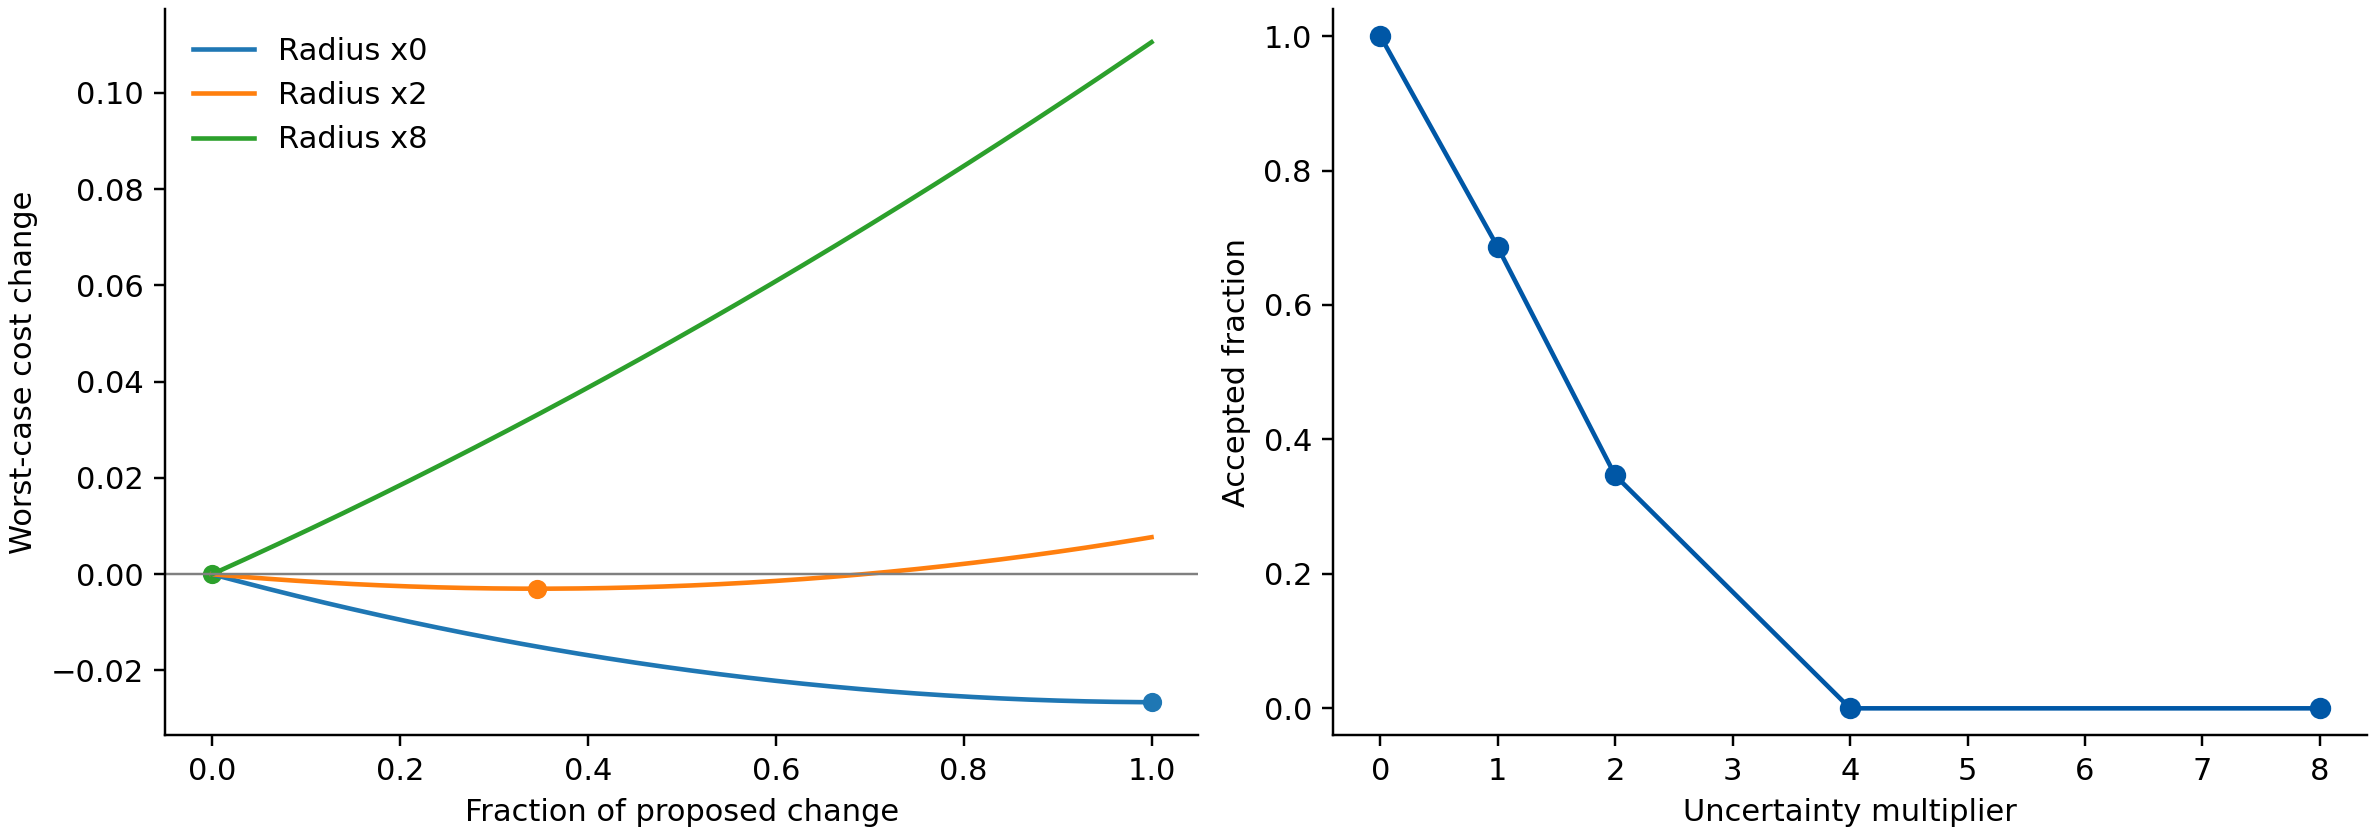
\includegraphics[width=0.94\linewidth]{figures/12_certified_improvement.png}
\caption{A proposal can have a negative nominal cost change and an adverse
worst-case change. The accepted fraction minimizes the exact common-model
comparison. The right panel shows how increasing uncertainty contracts the
accepted change. Synthetic model; no market observations.}
\label{fig:certifiedexecution}
\end{figure}

For a market study, freeze the baseline, candidate-generation rule,
uncertainty calibration and execution horizon before evaluating orders.
Report both the realized shortfall difference and how often the certificate
accepts a change. Separate failures of coefficient coverage, executable
capacity, and ledger reconciliation from optimization error.
